
\documentclass[preprint,12pt]{elsarticle}

\usepackage[spanish]{babel}
\usepackage{amssymb}
\usepackage{graphicx}
\usepackage{lineno}
\usepackage[utf8]{inputenc}
\usepackage{url}
\usepackage{natbib}

\begin{document}
	
	\begin{frontmatter}

		\title{\huge  Comparativa de Cuadro de Mando Integral (BSC) y Modelo de Negocio Canvas (BMC) }
		\author{Robles Flores, Anthony Richard	                (2016056192)}
		\author{Estrella Palacios, Katherine Lizbeth			(2015050948)}
		\author{Sosa Bedoya, Sharon Fiorela				(2016054460)}
		\author{Torres Beltran , Johanna Andrea			(2020067849)}
		\address{Tacna, Perú}
		


%%INICIO abstract
\begin{abstract}
The Balanced Scorecard (CMI Spanish Acronym) and the Canvas model can be linked as complementary tools for entrepreneurs. The first develops goals and operational measures in four main perspectives for the purpose of achieving the mission and strategy. The second suggest a (re-) evolution in generating business models, establishing nine sections that reflect their logic. In the article a working model is developed that, based on the need for a CMI it relates its design to the information previously collected in the Canvas model, pointing their mutual necessity
\end{abstract}
%%FIN abstract


\end{frontmatter}

%%INICIO Resumen
\section{Resumen}
El Cuadro de Mando Integral (BSC) y el modelo Canvas pueden enlazarse como herramientas complementarias para los emprendedores. La primera desarrolla objetivos y medidas operativas en cuatro perspectivas principales para alcanzar la misión y estrategia. La segunda ha supuesto una (re-)evolución en la generación de modelos de negocio, estableciendo nueve apartados que reflejan su lógica. En el artículo se desarrolla un modelo de trabajo que, partiendo de la necesidad de disponer de un BSC, relaciona su diseño con la información recogida previamente en el modelo Canvas, señalando su mutua necesidad.
%%FIN Resumen


%%INICIO Introducción
\section{Introducción}



%%FIN Introducción


%%INICIO Marco Teórico
\section{Marco Teórico}

%%----------------------------------------------------------------------------------------------------------------------------------------------------------
	\subsection{\textbf{Cuadro de Mando Integral (BSC)}}
	
xxxxxxxxxxxxxxxxxxxxxxxxxxxxxxxxxxxxxxxxxxxxxxxxxxxxxxxxxxxxxxxxxxxxxxxxxxxxxxxxxxxxxxxxxxx\cite{referenciarobles1}

\subsubsection{\textbf{Subtitulo 1}}

	\begin{itemize}
	\item a
	\item b
	\item c
	\end{itemize}



\subsubsection{\textbf{Subtitulo 2}}

	\begin{itemize}
	\item a
	\item b
	\item c
	\end{itemize}

%%----------------------------------------------------------------------------------------------------------------------------------------------------------

	\subsection{\textbf{Modelo de Negocio Canvas (BMC) }}
	
xxxxxxxxxxxxxxxxxxxxxxxxxxxxxxxxxxxxxxxxxxxxxxxxxxxxxxxxxxxxxxxxxxxxxxxxxxxxxxxxxxxxxxxxxxxxxxxxxxxxxxxxxxxx

	\subsubsection{\textbf{Subtitulo 1}}
	\begin{itemize}
	\item{\textbf{1. Punto1: }}XXXXXXXXXXXXX
	\item {\textbf{2. Punto2: }}XXXXXXXXXXXX
	\item {\textbf{3. Punto3: }}XXXXXXXXXXXX
	\end{itemize}

	\subsubsection{\textbf{Subtitulo 2}}

	\begin{itemize}
	\item a
	\item b
	\item c
	\end{itemize}

	\subsubsection{\textbf{Subtitulo 3}}

	\begin{figure}[htb]
		\begin{center}
			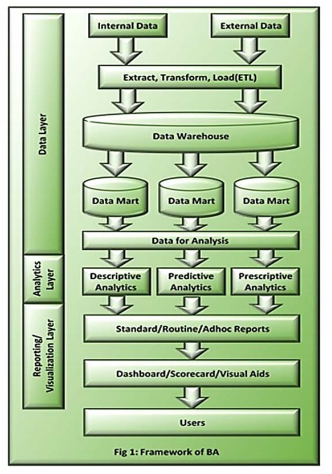
\includegraphics[height=9cm]{./IMAGENES/BAFramework} 
			\caption{Framework de BA}
		\end{center}
	\end{figure}


%%FIN Marco Teórico
%%----------------------------------------------------------------------------------------------------------------------------------------------------------


%COMPRACION

\section{Comparación entre Cuadro de Mando Integral (BSC) y Modelo de Negocio Canvas (BMC)}
A continuación se muestra la comparación entre Cuadro de Mando Integral (BSC) y Modelo de Negocio Canvas (BMC)
	
	\begin{itemize}

	\item{\textbf{1.}} XXXXXXXXXXXXXXXXXXXX
	\item{\textbf{2.}} XXXXXXXXXXXXXXXXXXXX
	\item{\textbf{3.}} XXXXXXXXXXXXXXXXXXXX
	\item{\textbf{4.}} XXXXXXXXXXXXXXXXXXXX
	\item{\textbf{5.}} XXXXXXXXXXXXXXXXXXXX
	\item{\textbf{6.}} XXXXXXXXXXXXXXXXXXXX
	\item{\textbf{7.}} XXXXXXXXXXXXXXXXXXXX
	\end{itemize}

%%----------------------------------------------------------------------------------------------------------------------------------------------------------

%CONCLUSIONES
\section{Conclusiones}

%%****
	\begin{itemize}
		\item XXXXXXXXXXXXXXXXXXXX
		\item XXXXXXXXXXXXXXXXXXXX
		\item XXXXXXXXXXXXXXXXXXXX
	\end{itemize}

%%----------------------------------------------------------------------------------------------------------------------------------------------------------

%RECOMENDACIONES
\section{Recomendaciones}	

	\begin{itemize}
		\item XXXXXXXXXXXXXXXXXXXX
		\item XXXXXXXXXXXXXXXXXXXX
		\item XXXXXXXXXXXXXXXXXXXX
	\end{itemize}


%%----------------------------------------------------------------------------------------------------------------------------------------------------------

	
	\newpage
	\bibliographystyle{apalike}
	\bibliography{BIBLIOGRAFIA}	



\end{document}

